\documentclass{article}



%% For IPA  
\usepackage{tipa}


%% for xeCJK
\usepackage{xeCJK}
\setCJKmainfont{SimSun}

\usepackage{xcolor}
\usepackage{hyperref}

\usepackage{amsmath}
\usepackage{pgf}
\usepackage{tikz}
\usetikzlibrary{arrows,shapes,snakes,automata,backgrounds,petri,matrix,arrows,arrows,%
    decorations.pathmorphing,decorations,backgrounds,decorations.text,%
    decorations.fractals,shadows,patterns,fadings,shapes,through,fit,positioning,scopes%
    }


%% title and author
\title{The Analysis of Hpeg}
\author{李约瀚 \\ 14130140331 \\ me@qinka.pro \\ qinka@live.com}

\begin{document}

%% title and table of content
\maketitle
\newpage
\tableofcontents
\newpage

%% Summary
\section{Summary}
\label{sec:summary}












%% Hpeg
\section{Hpeg}
\label{sec:hpeg}

\subsection{About}
\label{sec:hpeg:about}

Hpeg(\textipa{/"eItS""pEg/}) is another jpeg-like method of compression for digital images, written by me.
Hpeg is using DCT(Discrete Cosine Transform) as lossy compression method, and spare matrix as the entropy coding method.
Meanwhile, the final datas are compressed with lzma compression algorithm for using spare matrix to code. 

The project Hpeg's codes had been already opened on \href{http://github.com/Qinka/hpeg.hs}{GitHub}.
Until now, however, there is not any document for this project but just some comment in Haddock.
Hpeg is written in Haskell, and its algorithms are design for running on the GPU with many computing unit.
That program can run with a GPU which supports CUDA,and it use library \href{https://github.com/AccelerateHS/accelerate}{accelerate}.
But unfortunately, building this program might be an ugly thing.

The program take a Window BMP image as input and will output the .hpeg file,
and it also take a .hpeg as input and output a Window BMP image with RGBA\footnote{For A in the RGBA, is constant 0xFF}.

\subsection{Inside}
\label{sec:hpeg:inside}

Hpeg is using DCT and spare matrix, and now let's talk about the general workflow of encoding to Hpeg. The first thing to do is reading from the .bmp file.
Next, the colors under RGB need to be convert to YCbCr, because when using DCT the color space YCbCr will be used. 
Then the luminance and chroma will be transformed by DCT. Then the transformed matrix will be encoded with spare matrix.
Finally, the encoded one will be stored on the disk. However the data will be compressed with LZMA before it's stored.

So the decoding is similar with encoding. The first thing to do is reading from file, and constructing from spare matrix.
Next, matrix transform with IDCT(Inverse Discrete Cosine Transform). After the colors under YCbCr got, the colors will be convert
back to RGB. Finally, the datas will be written into a .bmp file. The figure \ref{fig:hpeg:workflow} might be more visual.

\begin{figure}
    \centering
    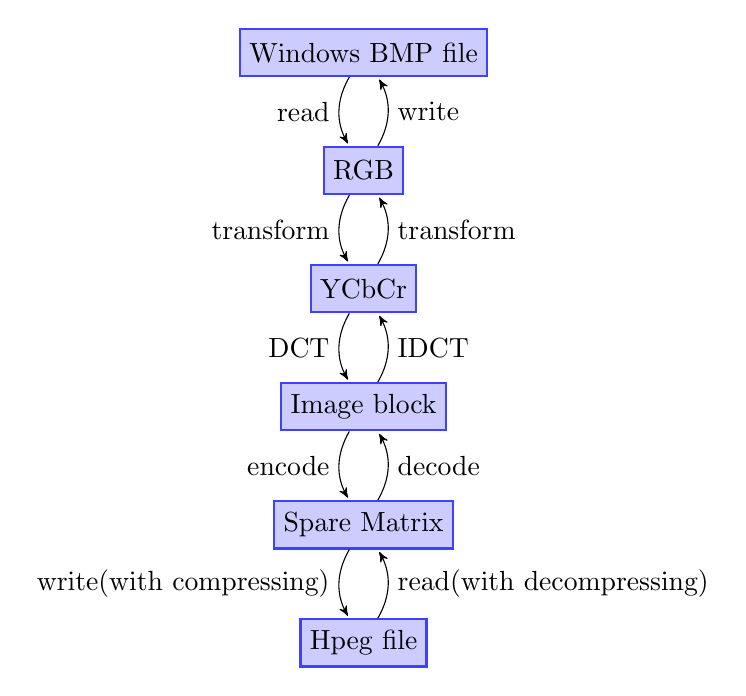
\begin{tikzpicture}[node distance=1.5cm,>=stealth',bend angle=30,auto]
        \tikzstyle{point}=[rectangle,thick,draw=blue!75,fill=blue!20,minimum size=6mm]
        \begin{scope}
        \node[point](bmp){Windows BMP file};
        \node[point](rgb)[below of=bmp]{RGB}
            edge [pre,bend left]   node         {read} (bmp)
            edge [post,bend right] node [right] {write}(bmp);
        \node[point](ycbcr)[below of=rgb]{YCbCr}
            edge [pre,bend left]   node         {transform}(rgb)
            edge [post,bend right] node [right] {transform}(rgb);
        \node[point](ib)[below of=ycbcr]{Image block}
            edge [pre,bend left]   node         {DCT}(ycbcr)
            edge [post,bend right] node [right] {IDCT}(ycbcr);
        \node[point](sm)[below of=ib]{Spare Matrix}
            edge [pre,bend left]   node         {encode}(ib)
            edge [post,bend right] node [right] {decode}(ib);
        \node[point](hpeg)[below of=sm]{Hpeg file}
            edge [pre,bend left]   node         {write(with compressing)}(sm)
            edge [post,bend right] node [right] {read(with decompressing)}(sm);
        \end{scope}
    \end{tikzpicture}
    \caption{Workflow of Hpeg Encoding and Decoding}
    \label{fig:hpeg:workflow}
\end{figure}

\subsubsection{Convertion for Color Space}
\label{sec:hpeg:inside:cfcs}

The first task in encoding and decoding is converting between two color spaces: RGB, and YCbCr.
The Eq.\ref{eq:colorspaceconvert1} and Eq.\ref{eq:colorspaceconvert2} are the equations for converting
between RGB and YCbCr, where $R,G,B \in \left[0,255\right]$ mean ``red'', ``blue'', and ``green'',
and $Y \in \left[-15,15\right]$ and $Cb,Cr \in \left[-127,127\right]$ mean ``luminance'', blue-diff chroma component, and red-diff chroma component.
\begin{equation}
    \label{eq:colorspaceconvert1}
    \left\{\begin{array}{rcl}
    Y  &=& 0.257R+0.564G+0.098B+16 \\
    Cb &=& -0.147R-0.291G+0.439B+128 \\
    Cr &=& 0.439R-0.368G-0.071B+128
    \end{array}\right.
\end{equation}
\begin{equation}
    \label{eq:colorspaceconvert2}
    \left\{\begin{array}{rcl}
    R &=& 1.164(Y-16) + 1.596(Cr-128) \\
    G &=& 1.164(Y-16) - 0.392(Cb-128)-0.813(Cr-128) \\
    B &=& 1.164(Y-16) + 2.017(Cb-128)
    \end{array}\right.
\end{equation}

So with Eq.\ref{eq:colorspaceconvert1} and Eq.\ref{eq:colorspaceconvert2},
the matrices of color will be convert between RGB and YCbCr in GPU.

\subsubsection{DCT \& IDCT}
\label{sec:hpeg:inside:dct}

After the colors converted to YCbCr color space, the matrices of the color need to be transformed with DCT.
Meanwhile, before the colors converted to RGB in decoding, the matrices of the color need to be transformed
with IDCT.

For 2D Discrete Cosine Transformation, its equation is Eq.\ref{eq:dct2}.
\begin{equation}
\label{eq:dct2}
F(u,v) = \frac{2C(u)C(v)}{\sqrt{MN}}\sum\limits_{i=0}^{M-1}\sum\limits_{j=0}^{N-1}\cos{\frac{(2i+1)u\pi}{2M}}\cos{\frac{(2j+1)v\pi}{2N}}f(i,j)
\end{equation}
where $i,u=0,1,\cdots,M-1$,$j,v=0,1,...,N-1$, and the constants $C(u)$ and $C(v)$ are determined by
\begin{equation}
\label{eq:2dct}
C(\xi) = \left\{
\begin{array}{cc}
\frac{\sqrt{2}}{2} & \xi = 0, \\
1 & otherwise.
\end{array}\right.
\end{equation}
Meanwhile the Eq.\ref{eq:idct2} is the 2D Inverse Discrete Cosine Transform.
\begin{equation}
\label{eq:idct2}
\widetilde{f}(i,j) = \sum\limits_{u=0}^{M-1}\sum\limits_{v=0}^{N-1}\frac{2C(u)C(v)}{\sqrt{MN}}\cos{\frac{(2i+1)u\pi}{2M}}\cos{\frac{(2j+1)v\pi}{2N}}F(i,j)
\end{equation} 

For both DCT and IDCT, the baisc unit is a $8 \times 8$ block, and each block is independent with other block.

\subsubsection{Spare Matrix}
\label{sec:hpeg:inside:sparematrix}

In the each block, the matrix transformed with DCT need to be quantized and encoding, when encoding.
It is similar in decoding. And the tables for quantization are table \ref{tab:luminacequantization} and
table \ref{tab:chromonacequantization}.

\begin{table}
    \centering
    \caption{The luminance quantization table.}
    \begin{tabular}{rrrrrrrr}
        \hline
        16 & 11 & 10 & 16 & 24 & 40 & 51 & 61 \\ 
        12 & 12 & 14 & 19 & 26 & 58 & 60 & 55 \\ 
        14 & 13 & 16 & 24 & 40 & 57 & 69 & 56 \\ 
        14 & 17 & 22 & 29 & 51 & 87 & 80 & 62 \\ 
        18 & 22 & 37 & 56 & 68 & 109 & 103 & 77 \\ 
        24 & 35 & 55 & 64 & 81 & 104 & 113 & 92 \\ 
        49 & 64 & 78 & 87 & 103 & 121 & 120 & 101 \\ 
        72 & 92 & 95 & 98 & 112 & 100 & 103 & 99 \\
        \hline
    \end{tabular}
    \label{tab:luminacequantization}
\end{table}

\begin{table}
    \centering
    \caption{The chromonace quantization table.}
    \begin{tabular}{rrrrrrrr}
        \hline
        17 & 18 & 24 & 47 & 99 & 99 & 99 & 99 \\ 
        18 & 21 & 26 & 66 & 99 & 99 & 99 & 99 \\ 
        24 & 26 & 56 & 99 & 99 & 99 & 99 & 99 \\ 
        47 & 66 & 99 & 99 & 99 & 99 & 99 & 99 \\ 
        99 & 99 & 99 & 99 & 99 & 99 & 99 & 99 \\ 
        99 & 99 & 99 & 99 & 99 & 99 & 99 & 99 \\ 
        99 & 99 & 99 & 99 & 99 & 99 & 99 & 99 \\ 
        99 & 99 & 99 & 99 & 99 & 99 & 99 & 99 \\
        \hline
    \end{tabular} 
    \label{tab:chromonacequantization}
\end{table}

The operation of the quantization is:
\begin{equation}
\label{eq:quantization}
\widehat{F}(u,v) = round\left(\frac{F(u,v)}{Q(u,v)}\right)
\end{equation}
where $F(u,v)$ is the transformed matrix, and $Q(u,v)$ is the matrix of the quantization.

For decoding, Eq.\ref{eq:quantization} will not work, and the following is needed:
\begin{equation}
\label{eq:iquantization}
F(u,v) = \left(\widehat{F}(u,v) \times Q(u,v)\right)
\end{equation}

After quantizing, the matrix will be represent with spare matrix.
The elements in the representation are index and the value. The higher 4-bit of the index is for ``u'',
and the lower 4-bit of the index is for ``v'', where $u$ and $v$ are the one in the Eq.\ref{eq:dct2}.
Both of the higher part and lower part's highest bit is reserved, for $u,v \in \left[0,7\right]$.

An item, a tuple of index and value, holds a non-zero element in the matrix.
And a list or array of the items represent a $8 \times 8$ matrix.
Then a list of array of the matrices represent a image or just say colors.

\subsubsection{Store}
\label{sec:hpeg:inside:store}

So till now, a Hpeg image includes the height, weight, Y's matrices, Cb's matrices, and Cr's matrices.
Meanwhile, Hpeg file also has a magic number at the beginning of the file -- "HpEg" in ASCII.

All this things will be serialized to or deserialized from bytes, as well as them will be written to or
read from the file.

\subsection{Codes}
\label{sec:hpeg:codes}

The codes of Hpeg has 5 modules. And they are organized as what figure \ref{fig:hpeg:layout} showed.

\begin{figure}
    \centering
    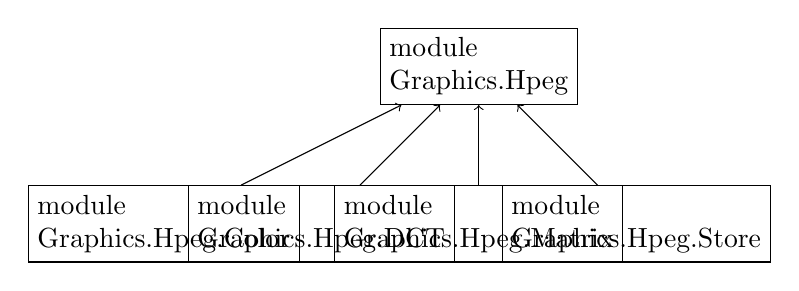
\begin{tikzpicture}[baseline=-.3em]
    \path
        (0,0)       node[draw,rectangle] (gh){\vbox{\hbox{module}\hbox{Graphics.Hpeg}}}
     ++ (-4,-2)     node[draw,rectangle] (ghc){\vbox{\hbox{module}\hbox{Graphics.Hpeg.Color}}}
     ++ (2,0)       node[draw,rectangle] (ghd){\vbox{\hbox{module}\hbox{Graphics.Hpeg.DCT}}}
     ++ (2,0)       node[draw,rectangle] (ghm){\vbox{\hbox{module}\hbox{Graphics.Hpeg.Matrix}}}
     ++ (2,0)       node[draw,rectangle] (ghs){\vbox{\hbox{module}\hbox{Graphics.Hpeg.Store}}}
     ;
     \draw [->] (ghc)--(gh);
     \draw [->] (ghd)--(gh);
     \draw [->] (ghm)--(gh);
     \draw [->] (ghs)--(gh);
    \end{tikzpicture}
    \caption{The layout of the Hpeg's codes}
    \label{fig:hpeg:layout}
\end{figure}

The codes in module \verb|Graphics.Hpeg.Color| convert the colors between the different color spaces.
The module \verb|Graphics.Hpeg.DCT| is about the DCT.
The module \verb|Graphics.Hpeg.Matrix| is about transforming or converting between different kinds of representation of matrix.
The module \verb|Graphics.Hpeg.Store| is about the form when store the data.
The module \verb|Graphics.Hpeg| is encapsulation of all the method, which convert the images between the Windows BMP and Hpeg.







%% test
\section{Test}
\label{sec:test}












%% improvement
\section{Improvement}
\label{sec:improvement}

\end{document}